\documentclass[t]{beamer}

\usepackage[english]{babel}
\usepackage[utf8]{inputenc}
\usepackage[T1]{fontenc}

\usepackage{amsmath}
\usepackage{amssymb}
\usepackage{float}
\usepackage{graphicx}
\graphicspath{{../images/}}
\usepackage{tikz}
\usepackage{hyperref}
\hypersetup{
    colorlinks,
    citecolor=black,
    filecolor=black,
    linkcolor=black,
    urlcolor=blue
}

\usetheme{metropolis}

\usepackage{lmodern}
\usepackage[scale=2]{ccicons}

\title{Data-driven Confocal Microscopy to Hematoxylin and Eosin Transformation}
\subtitle{Digitally Stained Confocal Microscopy through Deep Learning}
\author{Sergio García Campderrich}
%\institute{Universitat Politècnica de Catalunya}
\date{\today}

%% Custom commands
\newcommand{\cycleGAN}[2]{G_{#1 \rightarrow #2}}
\newcommand{\tensor}[1]{\mathbf{#1}}
\newcommand{\R}{\mathbb{R}}
\DeclareMathOperator*{\argmax}{arg\!\max}
\DeclareMathOperator*{\argmin}{arg\!\min}

\begin{document}
\setbeamertemplate{caption}{\raggedright\insertcaption\par}
\maketitle

\begin{frame}
\frametitle{Contents}

\begin{itemize}
\item Introduction\pause
\item Theoric background\pause
\item Methodology\pause
\item Experiments and results\pause
\item Conclusions and future development
\end{itemize}

\end{frame}


\AtBeginSubsection[]
  {
     \begin{frame}<beamer>
     \tableofcontents[currentsubsection,sections=\thesection]
     \end{frame}
  }

\section{Introduction}

\subsection{Hematoxylin and Eosin (H\&E)}

\begin{frame}
\frametitle{What is it?}

\begin{columns}

\begin{column}{0.5\textwidth}
\begin{figure}
\centering
\only<1->{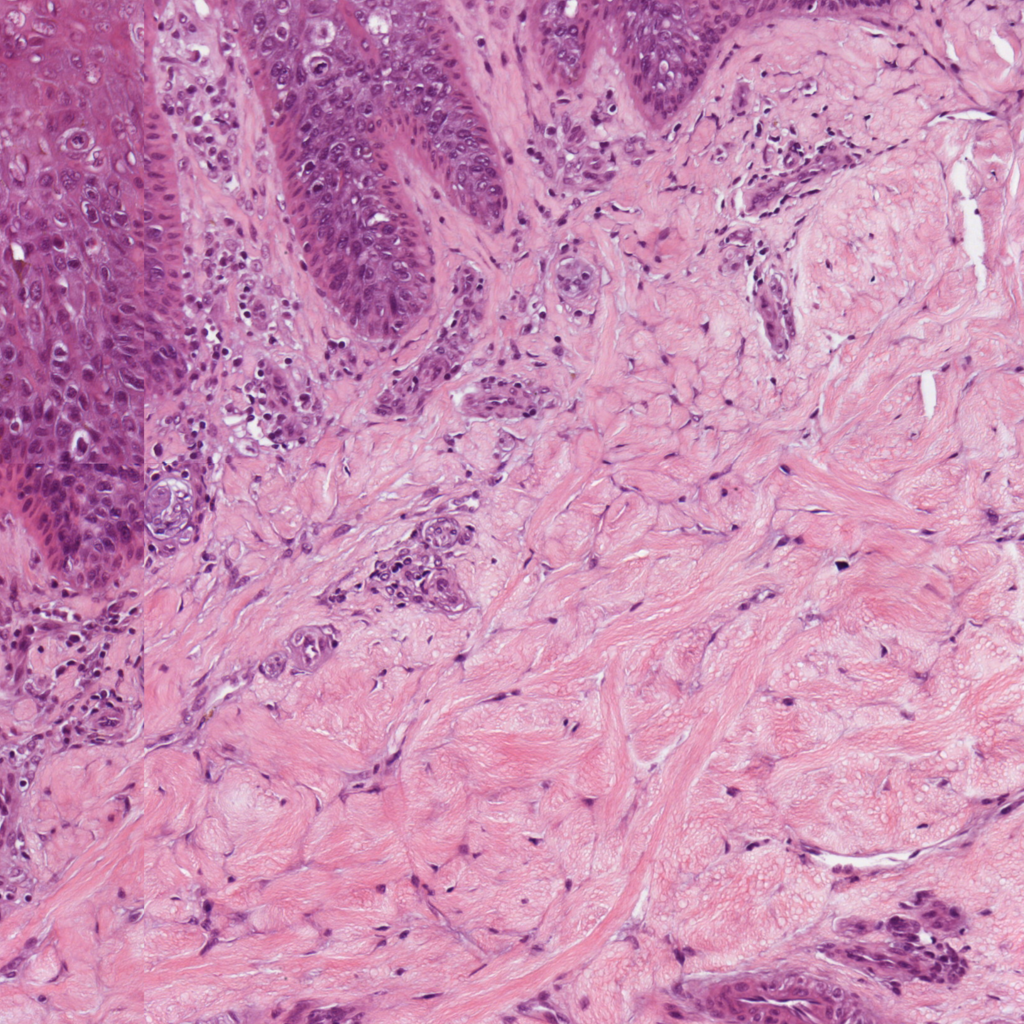
\includegraphics[width=0.9\textwidth]{HE-2}
\caption{H\&E stained tissue sample}}
\end{figure}
\end{column}\pause

\begin{column}{0.5\textwidth}
\only<2-3>{
\begin{block}{Usage}
\begin{itemize}
\item<2-3> Hematoxylin and eosin stain (H\&E stain) is one of the principal tissue stains used in histology and Mohs sugery.
\item<3> The \textbf{hematoxylin} stains cell nuclei \textbf{blue}, and \textbf{eosin} stains the
extracellular matrix and cytoplasm \textbf{pink}, with other structures taking on different shades, hues,
and combinations of these colors.
\end{itemize}
\end{block}
}
\only<4->{
\begin{alertblock}{It can be a slow process}
\begin{itemize}
\item<4-5> Tissues are typically frozen, cut, fixed in alcohol and then stained.
\item<5> Involves application of hematoxylin mixed with a metallic salt, a rinse in a weak acid solution, followed by bluing in alkaline water.
After the application of hematoxylin, the tissue is counterstained with eosin.
\end{itemize}
\end{alertblock}
}
\end{column}

\end{columns}
% La histología es la rama de la biología que estudia la composición, la estructura y las características de los tejidos orgánicos de los seres vivos.

% La cirugía de Mohs, es un tipo de cirugía microscópica controlada, altamente eficaz para tratar ciertos tipos comunes de cáncer de piel.
% controla micrográficamente, de manera que el paciente permanece en el quirófano mientras se estudia por microscopio el tejido extraído, proporciona el retiro exacto del tejido canceroso, mientras que se ahorra el tejido sano.
\end{frame}

\subsection{Confocal microscopy}

% La microscopía confocal es una tecnología que permite a los patólogos el análisis rápido de muestras de tejido para la detección de carcinomas.
% Sin embargo, esta tecnología aún no se ha establecido en la práctica clínica estándar porque la mayoría de los patólogos carecen del conocimiento para interpretar su salida.

\begin{frame}
\frametitle{What is it?}

CM is an optical imaging technique for increasing optical resolution and contrast of a micrograph
by means of using a spatial pinhole to block out-of-focus light in image formation.

It is able to capture multiple two-dimensional images at different depths in a sample (a process known as optical sectioning).

\begin{figure}
\centering
     \only<2>{
     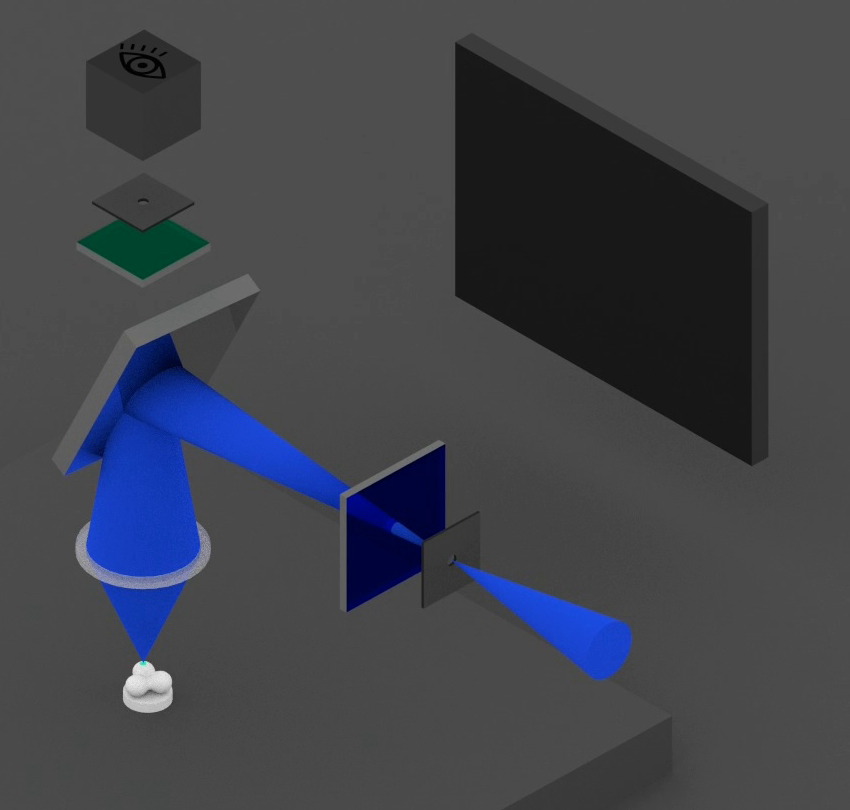
\includegraphics[scale=0.1]{CM-process-1-1}\hspace{0.1\textwidth}%
     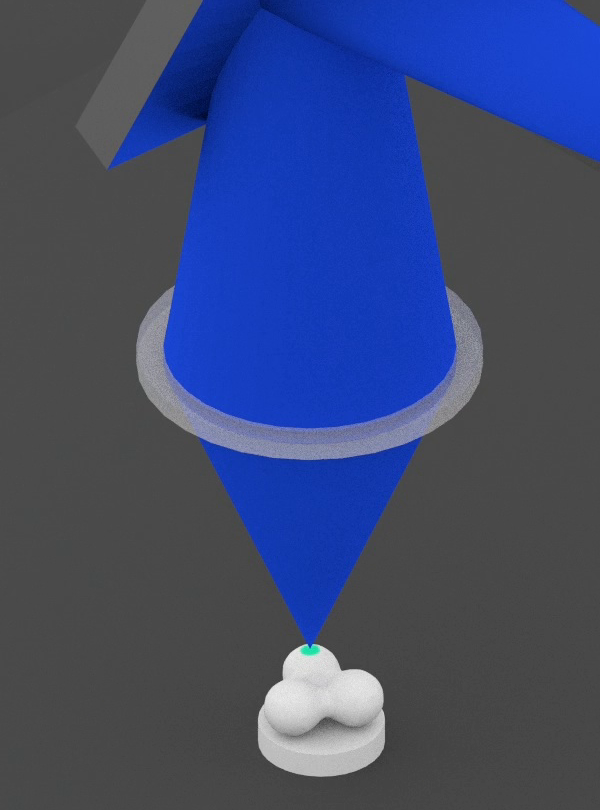
\includegraphics[scale=0.1]{CM-process-1-2}
     \caption{\footnotemark{}The light beam is focused by a pinhole on a small part of the sample}
     }
     \only<3>{
     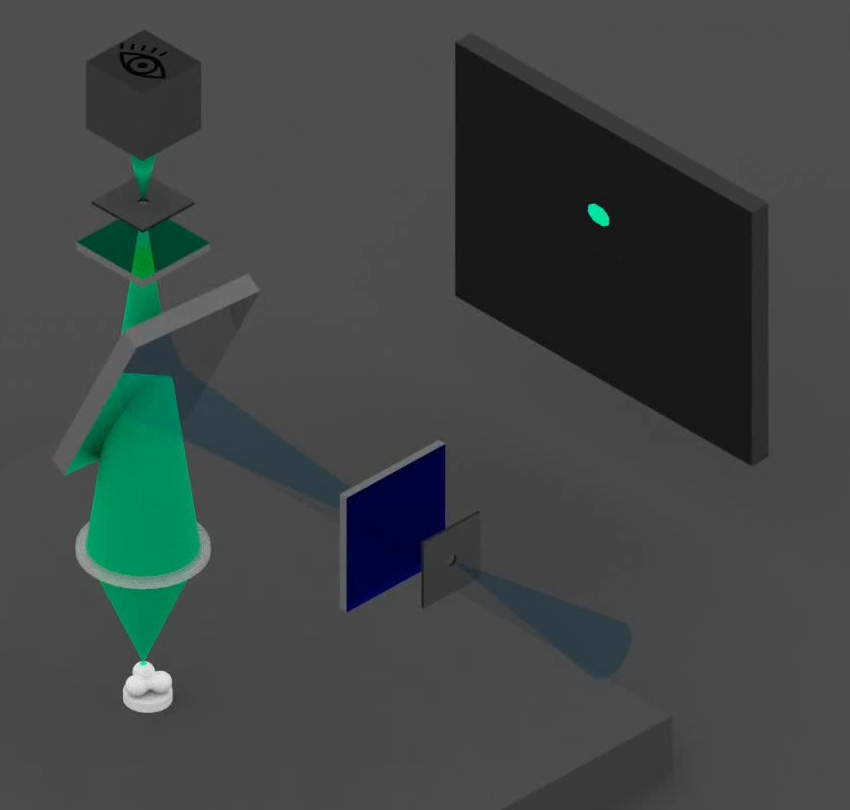
\includegraphics[scale=0.1]{CM-process-2-1}\hspace{0.1\textwidth}%
     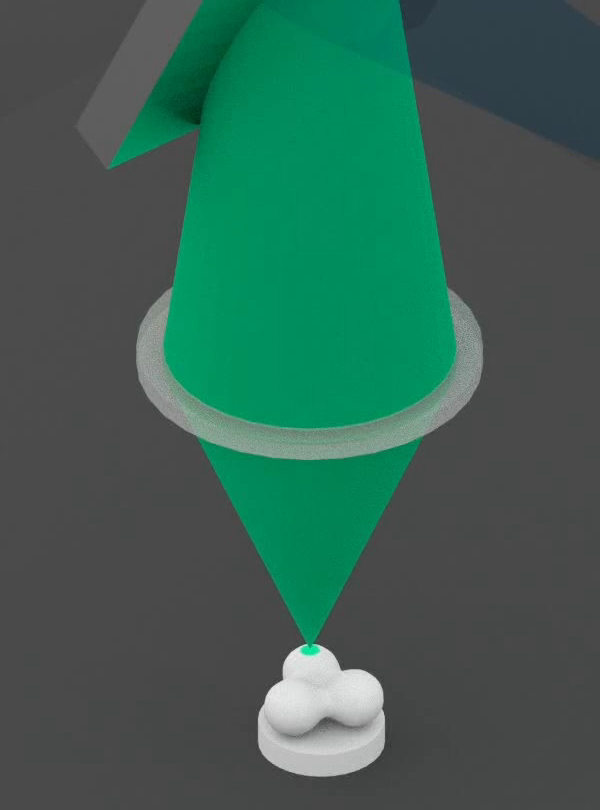
\includegraphics[scale=0.1]{CM-process-2-2}
     \caption{\footnotemark{}If fluorosphores are present, they emit light}
     }
     \only<4>{
     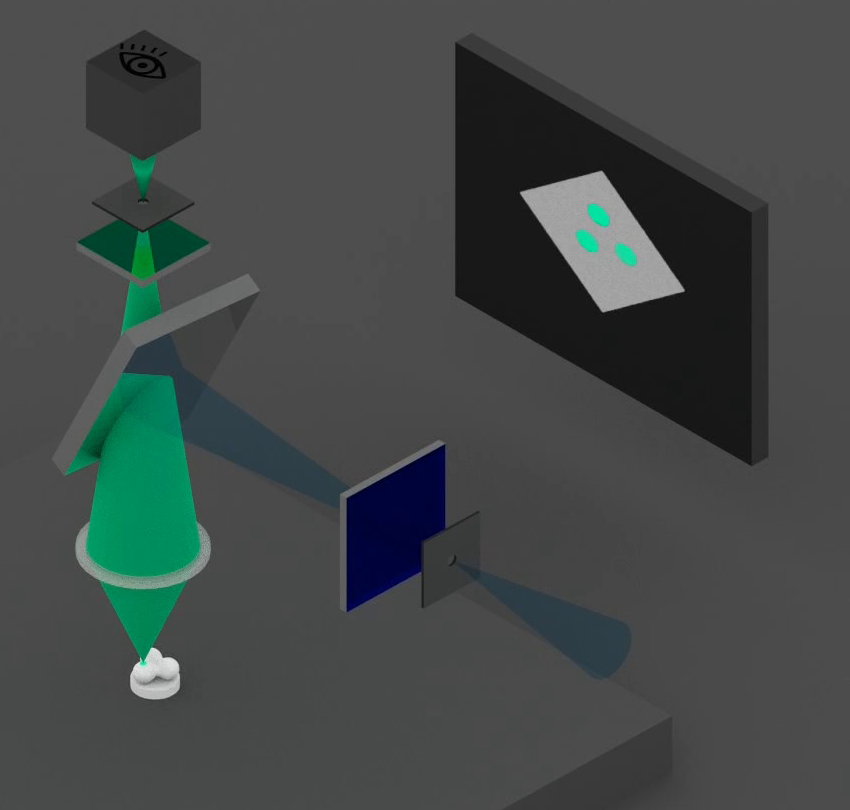
\includegraphics[scale=0.1]{CM-process-3-1}\hspace{0.1\textwidth}%
     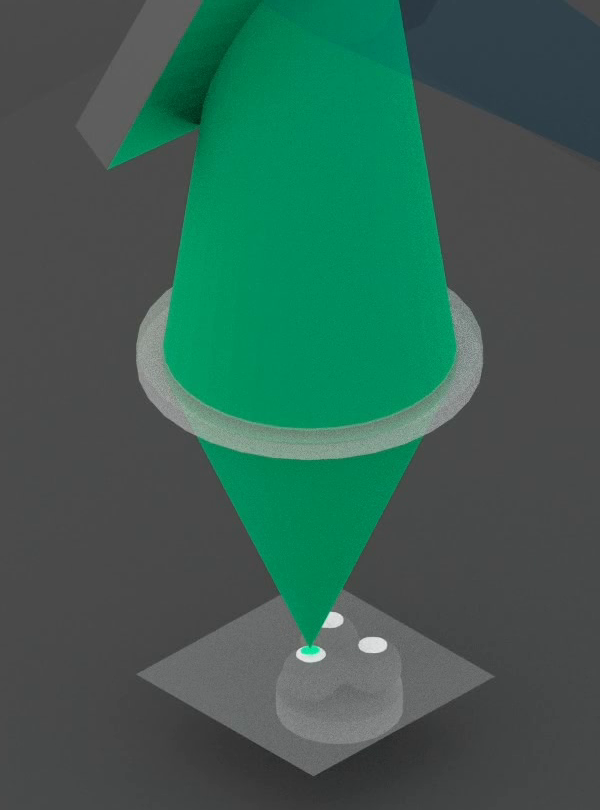
\includegraphics[scale=0.1]{CM-process-3-2}
     \caption{\footnotemark{}The surface is scanned by moving the sample/light beam}
     }
     \only<5>{
     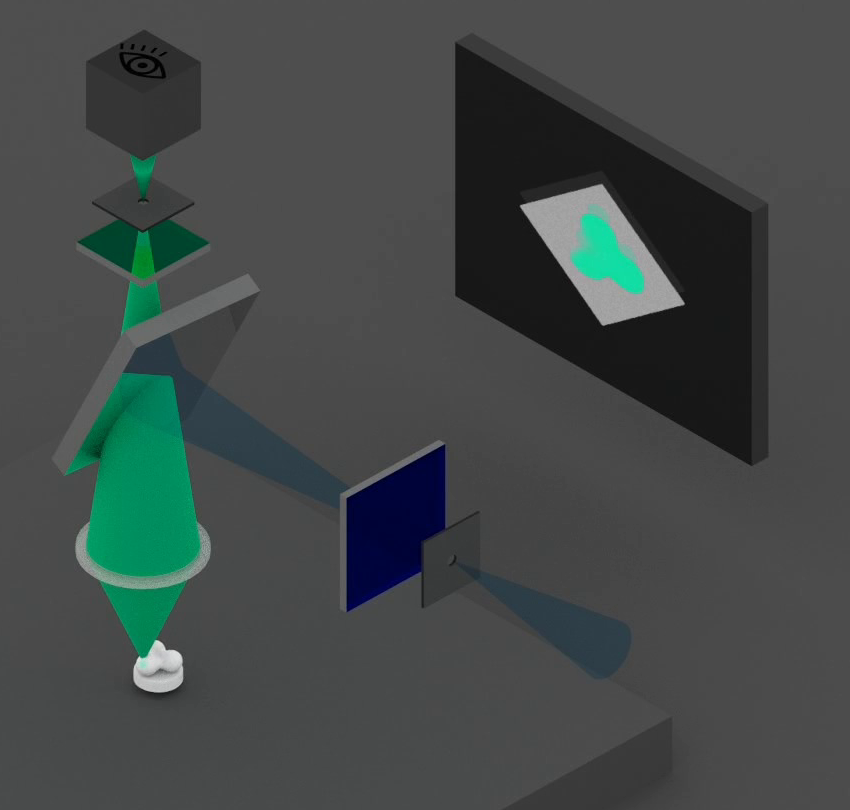
\includegraphics[scale=0.1]{CM-process-4-1}\hspace{0.1\textwidth}%
     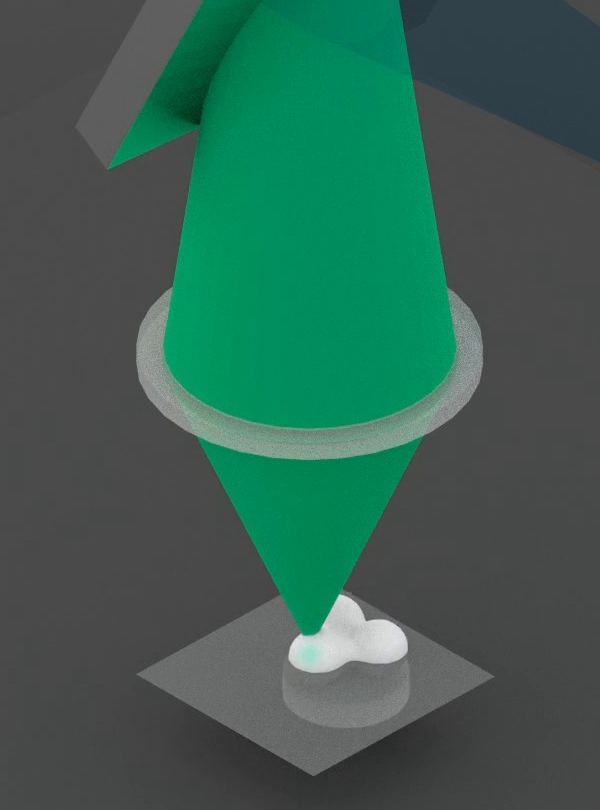
\includegraphics[scale=0.1]{CM-process-4-2}
     \caption{\footnotemark{}One can move vertically to obtain images at different heights}
     }
\end{figure}

\only<2->{
	\footnotetext{Images extracted from \href{https://commons.wikimedia.org/wiki/File:Fluorescent_and_confocal_microscopes.ogv}{wikimedia}.}
}

\end{frame}

\begin{frame}{Similarities and dissimilarities with H\&E}
    \begin{block}{Similarities}<1->
    {
        \begin{itemize}
        \item Usage in histopathology
        \item Up to cellular level resolution
	\item Expose similar structures in tissues
        \end{itemize}
    }
    \end{block}
    \begin{alertblock}{Differences}<2>
    {
        \begin{itemize}
        \item Specimens can be examined in near real-time without time consuming processing procedures.
        \item Output largely diers from the standard H\&E slides
        \end{itemize}
    }
    \end{alertblock}

\end{frame}

\begin{frame}{Modes}

In addition to ``standard'' reflection mode, CM can make use of fluorescent mode for specimens stained with fluorochromes.

\only<1>{
\begin{columns}

\begin{column}{0.5\textwidth}
\begin{figure}
\centering
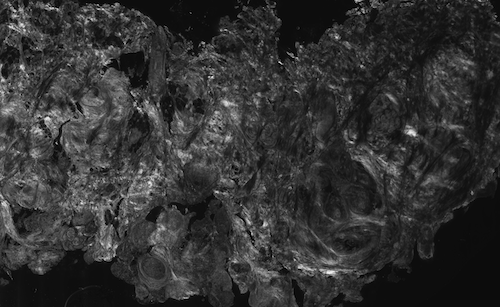
\includegraphics[width=0.9\textwidth]{CM-R}
\caption{Reflectance mode}
\end{figure}
\end{column}

\begin{column}{0.5\textwidth}
\begin{figure}
\centering
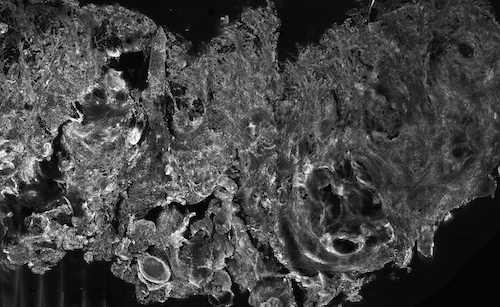
\includegraphics[width=0.9\textwidth]{CM-F}
\caption{Fluorescence mode}
\end{figure}
\end{column}
\end{columns}
}

\only<2>{
\begin{columns}

\begin{column}{0.5\textwidth}
\begin{figure}
\centering
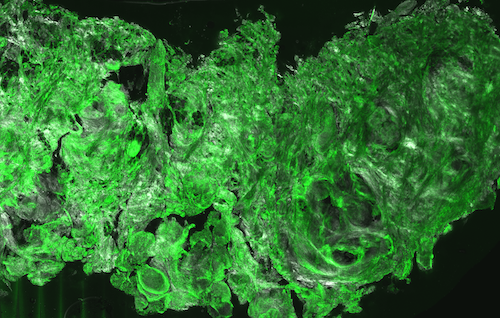
\includegraphics[width=0.9\textwidth]{CM-blend}
\caption{Blend of reflectance and fluorescence mode.}
\end{figure}
\end{column}

\begin{column}{0.5\textwidth}
\begin{figure}
\centering
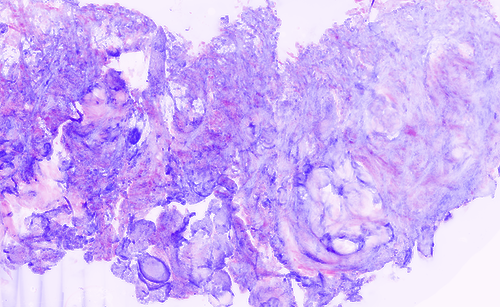
\includegraphics[width=0.9\textwidth]{CM-pseudocolor}
\caption{Pseudocolor/falsecolor H\&E-like from reflectance and fluorescence modes}
\end{figure}
\end{column}
\end{columns}
}


\end{frame}

\subsection{Data-driven transformation}

% Para abordar este problema, se presenta y evalúa un método basado en datos para transformar las micrografías confocales en imágenes parecidas a hematoxilina y eosina de aspecto más familiar, lo que permite a los patólogos interpretar estas imágenes sin formación específica.

\begin{frame}{Why?}
As confocal micrographs largely differ from the standard H\&E slides that
pathologists typically use to analyze tissue samples, professionals need
to undergo specific training.

A correctly done CM to H\&E mapping should bring the efficiency of CM
to untrained pathologists and surgeons.

\begin{columns}

\begin{column}{0.5\textwidth}
\begin{figure}
\centering
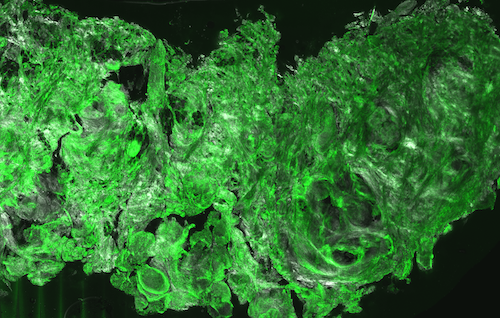
\includegraphics[width=0.9\textwidth]{CM-blend}
\end{figure}
\end{column}

\begin{column}{0.5\textwidth}
\begin{figure}
\centering
\includegraphics[scale=0.6]{doctor}
\end{figure}
\end{column}

\end{columns}
\end{frame}

\begin{frame}{Why?}
Standard pseudocolor transformation is a linear transformation that cannot capture the true appearance of H\&E stained samples.

Different structures should be mapped to different colours even if the pixel values are the same.

\begin{columns}

\begin{column}{0.5\textwidth}
\begin{figure}
\centering
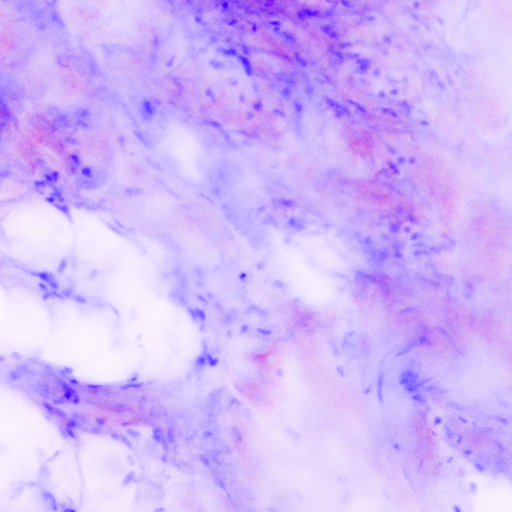
\includegraphics[width=0.5\textwidth]{epoch246_real_A}
\caption{Colors and structures greatly vary from the ones found in H\&E slides}
\end{figure}
\end{column}

\begin{column}{0.5\textwidth}
\begin{figure}
\centering
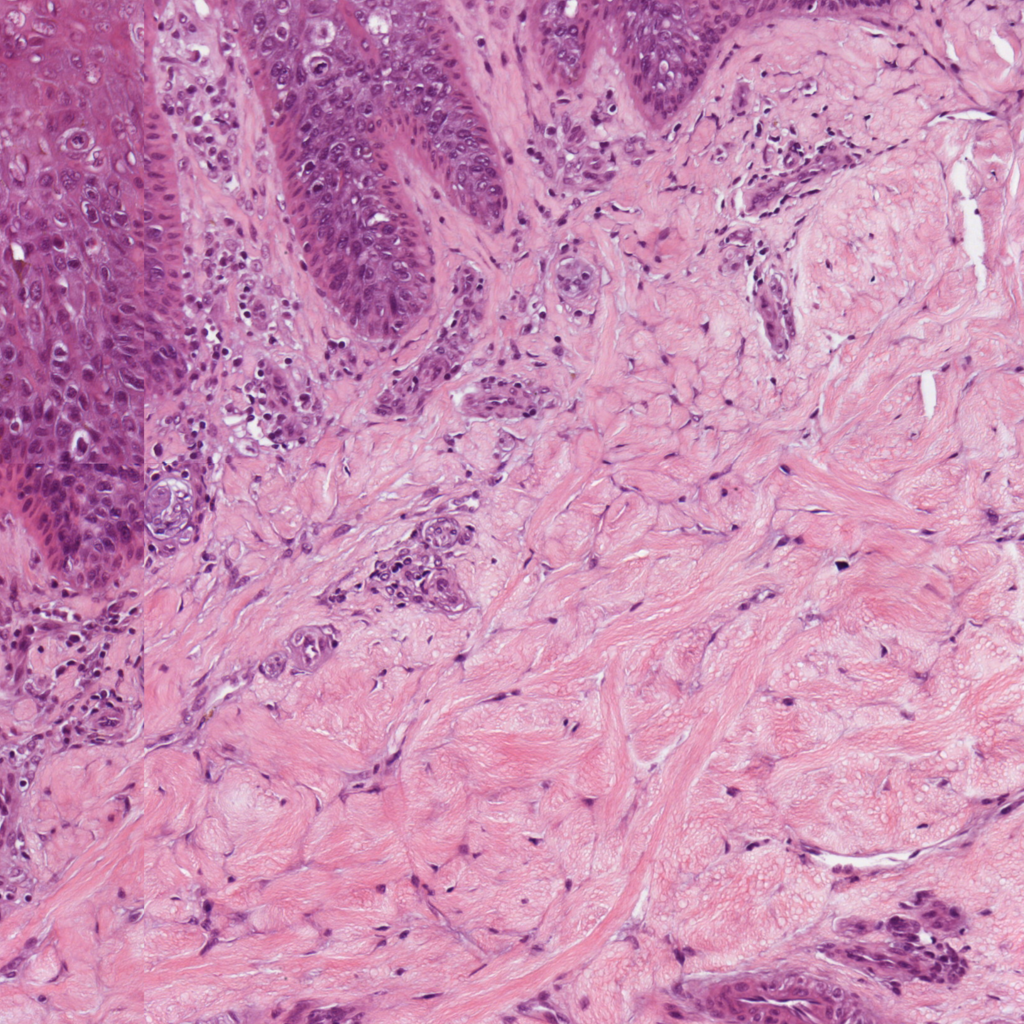
\includegraphics[width=0.5\textwidth]{HE-2}
\caption{H\&E slide}
\end{figure}
\end{column}

\end{columns}

\end{frame}

\begin{frame}{How?}
% El principal obstáculo para definir dicha transformación es la ausencia de datos confocales emparejados con imágenes de hematoxilina y eosina que necesitan los marcos tradicionales de aprendizaje automático. Para superar este problema, se utiliza el marco de redes generativas antagónicas de ciclo consistente.
% Este marco presenta problemas específicos como el entrenamiento inestable y la ``alucinación'' o eliminación de estructuras que este trabajo intenta cuantificar y mitigar.

\begin{figure}
\centering
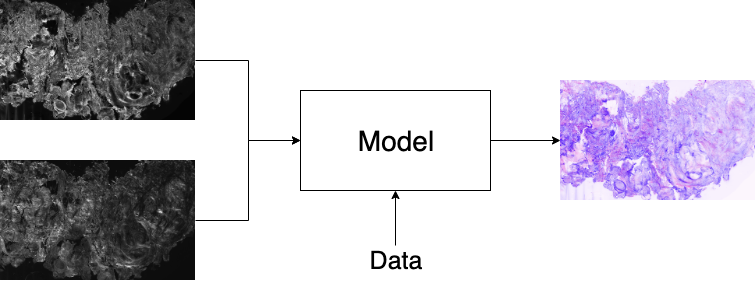
\includegraphics[width=0.5\textwidth]{transformation}
\end{figure}

\begin{columns}

\begin{column}{0.5\textwidth}
\begin{block}{Solution}
\begin{itemize}
\item<1-> Data driven approach to try to find a better transformation
\item<2-> Convolutional neural network are good at \emph{learning} non-linear mappings
\end{itemize}
\end{block}
\end{column}

\begin{column}{0.5\textwidth}
\begin{alertblock}{Problem}
\begin{itemize}
\item<3-> Traditional solutions would require pairs of CM and H\&E slides, which would be very difficult
\item<4-> Use of CycleGANs framework
\end{itemize}
\end{alertblock}
\end{column}


\end{columns}

\end{frame}


\section{Theoric background}

\subsection{Artificial neural networks}

\begin{frame}{Convolutional neural networks (CNNs)}

\begin{columns}

\begin{column}{0.4\textwidth}
\begin{tikzpicture}[baseline=(current bounding box.north)]
  \node (img1) {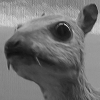
\includegraphics[width=0.3\textwidth]{conv-orig}};
  \onslide<2->{\node (img2) at (img1.north east) [xshift=0.25\textwidth] {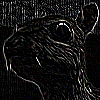
\includegraphics[width=0.3\textwidth]{conv-edge}};}
  \onslide<3->{\node (img3) at (img2.south east) {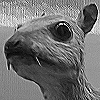
\includegraphics[width=0.3\textwidth]{conv-sharp}};}
  \onslide<4->{\node (img4) at (img3.south east) {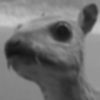
\includegraphics[width=0.3\textwidth]{conv-blur}};}
\end{tikzpicture}
\end{column}

\begin{column}{0.6\textwidth}
\begin{figure}
\onslide<5->{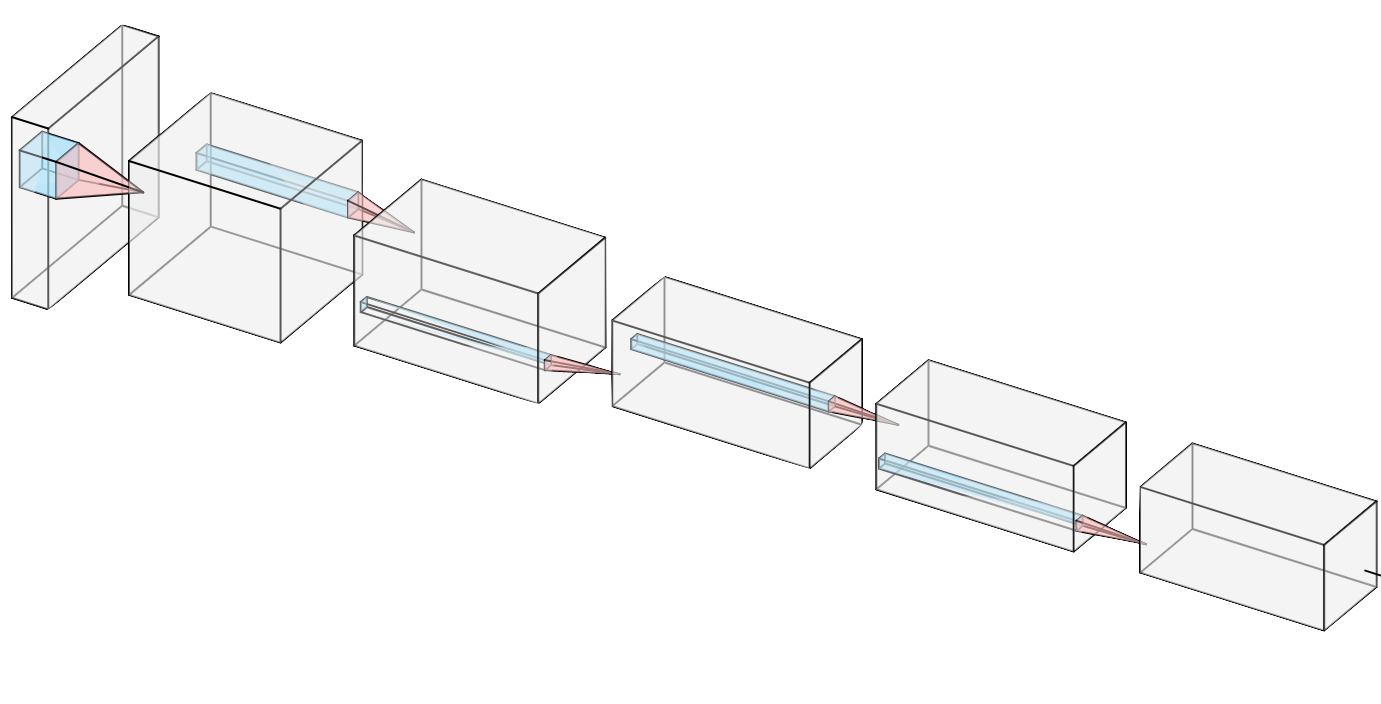
\includegraphics[width=0.8\textwidth]{fcnn}}
\end{figure}
\end{column}

\end{columns}

\begin{block}{Short description}
\begin{itemize}
\item Convolution is fast way to apply a linear translation-invariant transformation
\item<5-> A layer contains multiple filters
\item<5-> A layer's output is the concatenation of each resulting convolution
\end{itemize}
\end{block}

\end{frame}

\begin{frame}{Training}
% Differentiable by construction.
% Define an objective function a use gradient descent.
% Mention backpropagation algorithm.
% Defining an objective function for our problem is difficult (unpaired data)

\begin{block}{Define an objective function and optimize it}
\[
\theta^* = \argmin_{\theta} \mathcal{J}
\left( (\tensor{X}, \tensor{Y}), f_{\theta} \right)
\]

Neural networks are fully differentiable by construction, so we can use gradient-based methods.
\end{block}\pause

\begin{alertblock}{But}
Defining an objective function for our problem is straightforawrd.

We want to \emph{generate} images that \emph{look like} H\&E and are \emph{realistic}.
\end{alertblock}\pause

\begin{block}{Typically}
The objective function is defined as the expected value of a loss function that is applied to
a single data point
\[
\mathcal{J}\left( (\tensor{X}, \tensor{Y}), f_{\theta} \right) =
\mathbb{E}\{ \mathcal{L} \left( f_{\theta}(\tensor{X}), \tensor{Y} \right) \}
\]
\end{block}
\end{frame}

\subsection{Generative models}

\begin{frame}
\frametitle{Generative adversarial networks (GANs)}
% Quick and simple visual explanation.
Framework for estimating generative models via an adversarial
process, in which two models are trained: a generative model $G$ that captures
the data distribution, and a discriminative model $D$.

\begin{block}{Two-player minimax game}
\[
\min_G \max_D \mathbb{E}_{x \sim p_{data}(x)}\{\log D(x)\} +
\mathbb{E}_{z \sim p_z(z)} \{\log(1 - D(G(z)))\}
\]
\end{block}\pause

\begin{block}{Loss functions}
\[
\mathcal{L}_G = \log(1 - D(G(\tensor{z})))
\]

$$
\mathcal{L}_D =
  \begin{cases}
    - \log(D(\tensor{x})), & \tensor{x} \sim p_{data} \\
    - \log(1 - D(\tensor{x})), & \tensor{x} \sim p_g
  \end{cases}
$$
\end{block}

\end{frame}

\begin{frame}[b]
\frametitle{Visual representation}
\begin{figure}
     \only<1>{
     
\includegraphics[scale=0.4]{GANs_animation-1}
     \caption{Discriminator predicts the probability of being ``real'' of a sample drawn from the dataset}
     }
     \only<2>{
     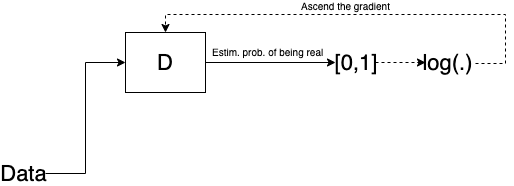
\includegraphics[scale=0.4]{GANs_animation-2}
     \caption{The discriminator's parameters are updated to increase the log-likelihood}
     }
     \only<3>{
     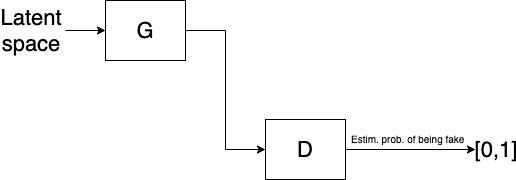
\includegraphics[scale=0.4]{GANs_animation-3}
     \caption{Discriminator predicts the probability of being ``fake'' of a sample drawn from the generator}
     }
     \only<4>{
     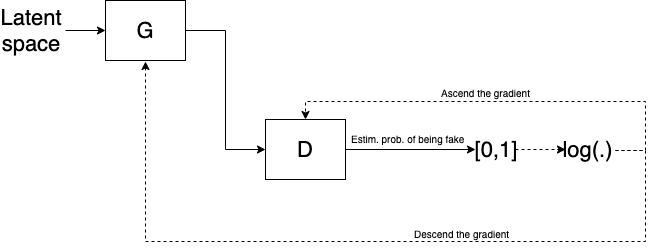
\includegraphics[scale=0.4]{GANs_animation-4}
     \caption{The discriminator's parameters are updated to increase the log-likelihood.
     The generator's parameters are updated to decrese the log-likelihood of the discriminator}
     }
\end{figure}

\end{frame}

\begin{frame}{Cicle-consistent GANs (CycleGANs)}
% Quick and simple visual explanation.
\only<1->{\begin{block}{Objective}
\begin{itemize}
\item Framework for image-to-image translation based on GANs, where
mapping is learned with unpaired data\pause

\item Unpaired data consists of a source set $\tensor{X}$ and a target set $\tensor{Y}$
with no information provided as to which $\tensor{x}_i$ matches which $\tensor{y}_i$
\end{itemize}
\end{block}
}

\only<2>{\begin{figure}
     \centering
     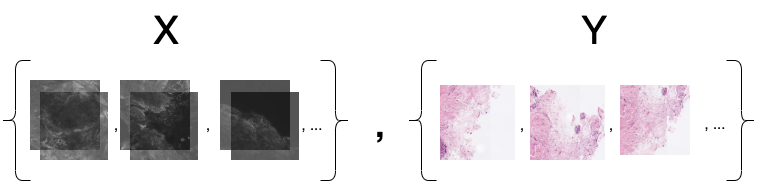
\includegraphics[scale=0.4]{unpaired_data}
\end{figure}
}
\only<3->{
\begin{alertblock}{Why not ``simple'' GANs?}
\begin{itemize}
\item<3-> Simply using the discriminator loss is not sufficient as it leads to the problem known as mode-collapse
where the generator ignores the source

\item<4-> This problem is addressed by ``encouraging'' the mapping to be cycle-consistent, i.e.:
$ \cycleGAN{Y}{X}(\cycleGAN{X}{Y}(\tensor{x})) \approx \tensor{x} $.
\end{itemize}
\end{alertblock}
}

\end{frame}

\begin{frame}
\frametitle{Cicle-consistent GANs (CycleGANs)}

\only<1->{
\begin{block}{Two pairs of generator-discriminator are trained}
\begin{itemize}
\item $\cycleGAN{X}{Y}$ maps from domain $X$ to domain $Y$. $D_Y$ discriminates in domain $Y$.
\item $\cycleGAN{Y}{X}$ maps from domain $Y$ to domain $X$. $D_X$ discriminates in domain $X$.
\end{itemize}
\end{block}
}

\only<2->{
\begin{columns}

\begin{column}{0.4\textwidth}
\begin{figure}
\centering
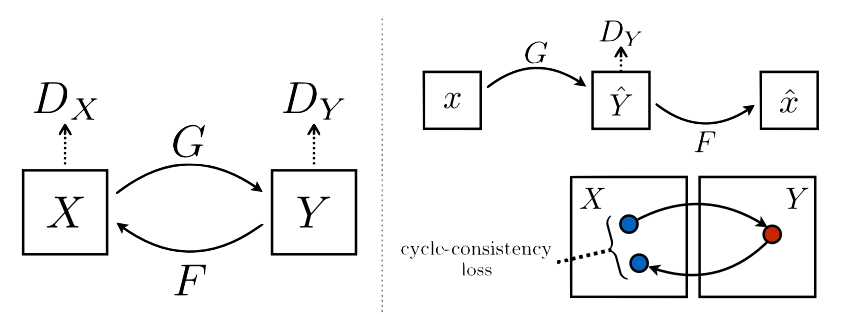
\includegraphics[width=\textwidth]{cyclegan-diagram-small}
\end{figure}
\end{column}

\begin{column}{0.6\textwidth}
\[
\begin{split}
\mathcal{L}_{\cycleGAN{X}{Y}} = &\log(1 - D_Y(\cycleGAN{X}{Y}(\tensor{x}))) \\
&+ \lambda \left\| \tensor{x} -
\cycleGAN{Y}{X}(\cycleGAN{X}{Y}(\tensor{x})) \right\|_1 \\
\end{split}
\]
\end{column}

\end{columns}
}

\end{frame}


\section{Methodology}

\subsection{Datasets}

\begin{frame}
\frametitle{Confocal dataset}
% Ejemplos de whole slide confocal
\end{frame}

\begin{frame}
\frametitle{H\&E}
% Ejemplos whole slide H&E
\end{frame}

\subsection{Despeckling}

\begin{frame}
\frametitle{Speckle noise}
% Que es?
% Modelo de ruido
% Ejemplo del dataset
\end{frame}

\begin{frame}
\frametitle{Despeckling network}
% Diagrama
% Distintos tipos
\end{frame}

\subsection{Stain}

\begin{frame}
\frametitle{Residual network}
% Diagram
\end{frame}

\begin{frame}
\frametitle{UNet-like network}
% Diagram
\end{frame}

\subsection{Inference technique}

\begin{frame}
\frametitle{Why?}
% Example of "naive" approach
\end{frame}

\begin{frame}
\frametitle{"no-overlap" method}
% Diagram
\end{frame}

\begin{frame}
\frametitle{"pyramid" method}
% Diagram
\end{frame}

\subsection{Quality measure}

\begin{frame}
\frametitle{SSIM}
\end{frame}


\begin{frame}
\frametitle{LBP}
% Diagrama del los 8 puntos (mirar explicacion computerphile)
\end{frame}


\section{Experiments and results}

\subsection{Despeckling}

\begin{frame}
\frametitle{Experiments}
% Set-up
\end{frame}

\begin{frame}
\frametitle{Results}
% Learning curves...
% Ejemplos resultados...
\end{frame}

\subsection{Stain}

\begin{frame}
\frametitle{Experiments}
% set-up
\end{frame}

\begin{frame}
\frametitle{Results}
% Learning curves...
% Ejemplos de transformacion a lo largo del entrenamiento
% Ejemplos resultados...
\end{frame}

\subsection{Inference technique}

\begin{frame}
\frametitle{Experiments}
% Se transforman 7 whole slides...
% Mostrar (algunos) ejemplos
\end{frame}

\begin{frame}
\frametitle{Results}
% Mostrar ejemplos transformados
% Box plots
\end{frame}


\section{Conclusions and future development}

\begin{frame}{Conclusions}
\end{frame}

\begin{frame}{Future development}
\end{frame}

\end{document}
